\subsection{文法解读}
接下来对文法进行具体解释:
\subsubsection{程序的解读}
\[
	\sym{program} \define 
		\sym{block}.
\]
这句定义了程序是由分程序加``$.$"组成,其中``$.$"可以判定程序的结束。
这句的语法图见 Figure~\ref{program}。
\begin{figure}[h]
\begin{center}
    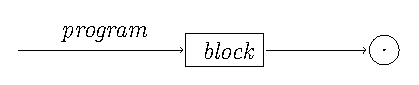
\includegraphics[scale=1]{Figures/program.eps}
\end{center}
\caption{program 语法图}
\label{program}
\end{figure}
具体实例:
\begin{verbatim}
count a = 2; .
\end{verbatim}
这就是一个完整的程序,``."表示程序的结束。
\subsubsection{分程序的解读}
\[
	\sym{block} \define 
		[\sym{constdec}] [\sym{vardec}] \{[\sym{procdec}] | [\sym{fundec}]\} \sym{compstmt}
\]
\[
	\sym{constdec} \define
		\keyword{const} \sym{constdef} \{,\sym{constdef}\};	
\]
\[
	\sym{constdef} \define
		\sym{ident} = \sym{const}
\]
\[
	\sym{vardec} \define
		\keyword{var} \sym{vardef}; \{ \sym{vardef}; \}
\]

\[
	\sym{vardef} \define
		\sym{ident}\{,\sym{ident}\}:\sym{type}
\]
\[
	\sym{procdec} \define
		\sym{prochead} \sym{block} \{; \sym{prochead} \sym{block} \};
\]
\[
	\sym{fundec} \define
		\sym{funhead} \sym{block} \{; \sym{funhead} \sym{block} \};
\]
\[
	\sym{prochead} \define
		\keyword{procedure} \sym{ident} '(' [\sym{paralist}] ')';
\]
\[
	\sym{funhead} \define
		\keyword{function} \sym{ident} '(' [\sym{paralist}] ')': \sym{basictype};
\]
\[
	\sym{compstmt} \define
		\keyword{begin} \sym{statement} \{; \sym{statement} \} \keyword{end}
\]
这几句定义了 \sym{block} 文法的完整视图,语法图见 Figure~\ref{block}。
\begin{figure}[!h]
\begin{center}
    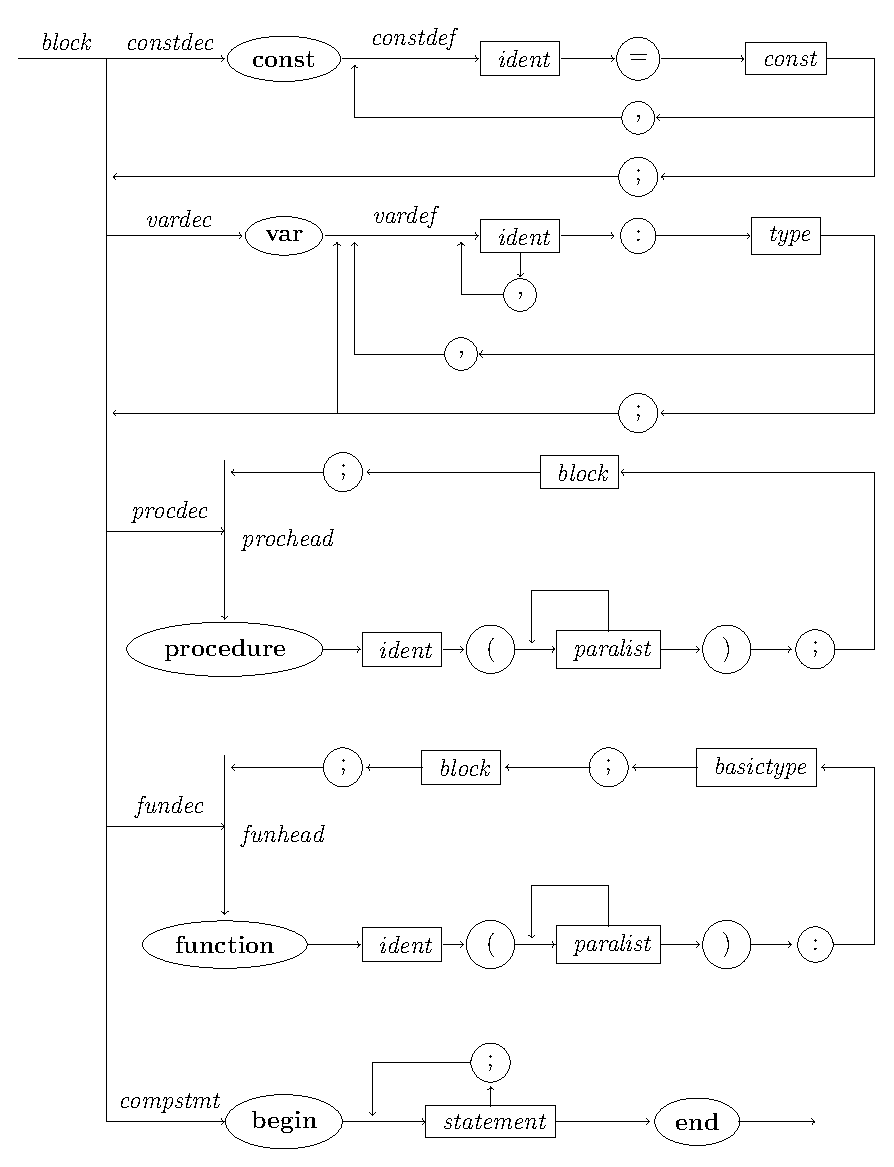
\includegraphics[scale=.8]{Figures/block.eps}
\end{center}
\caption{block 语法图}
\label{block}
\end{figure}
在分程序\sym{block}中先进行常量定义\sym{constdec},然后是变量定义
\sym{vardef} ,接着是过程的声明\sym{procdec}和函数声明\sym{fundec}
最终的\sym{block}通过一个复合语句\sym{compstmt}退出。\emph{这样的
顺序是不能改变的}。具体实例:
\begin{verbatim}
const numbera=0, numberb=1; // 常量定义
var i, j, sum: integer;     // 变量定义
procedure  test();          // 过程声明部分
  test 的程序(略)
function add():integer;     // 函数声明部分
begin
  sum := numbera + numberb; // add 的分程序部分
  add := sum
end;
                            // 复合语句部分
begin
  i := sum
end
\end{verbatim}
说明:
\begin{enumerate}
	\item 常量定义必须在变量前面,这种顺序不能改变。
		如: \verb|var i:integer;const a=1;|就是错误的。
	\item 相连的过程和函数的声明是可以打乱顺序的,过程和函数
		都可以右参数列表,用于传入参数。
	\item 常量是可以连续定义的,之间使用逗号隔开,最后以分号
		结束常量的定义.
	\item 变量的定义也可以连续定义,之间使用逗号隔开,另外使用冒号后跟
		变量类型来说明定义的变量的类型。变量的定义的结束是使用分号。
	\item 常量定义,变量定义,过程声明,函数声明对一个分程序来说是可有可无
		的,只有复合语句是必须部分。
\end{enumerate}
\subsection{语句的解读}
\[ \begin{aligned}
	\sym{statement} \define
		& \sym{assignstmt} | \sym{ifstmt} | \sym{repeatstmt} | \sym{pcallstmt} \\
		& \quad | \sym{compstmt} | \sym{readstmt} | \sym{writestmt} | \sym{forstmt} | \sym{nullstmt}
\end{aligned} \]

\[ \begin{aligned}
	\sym{assignstmt} \define
		& \sym{ident} := \sym{expression} | \sym{funident} := \sym{expression}  \\
		& \quad | \sym{ident} '[' \sym{expression} ']' := \sym{expression}
\end{aligned} \]
\[
\begin{aligned}
	\sym{ifstmt} \define
		& \keyword{if} \sym{condition} \keyword{then} \sym{statement} \\
		& \quad | \keyword{if} \sym{condition} \keyword{then} \sym{statement} \keyword{else} \sym{statement}
\end{aligned}
\]
\[
	\sym{repeatstmt} \define
		\keyword{repeat} \sym{statement} \keyword{until} \sym{condition}
\]
\[
	\sym{forstmt} \define
		\keyword{for} \sym{ident} := \sym{expression} ( \keyword{to} | \keyword{downto})
			\sym{expression} \keyword{do} \sym{statement}
\]
\[
	\sym{pcallstmt} \define
		\sym{ident} '(' [ \sym{arglist}] ')'
\]

\[
	\sym{compstmt} \define
		\keyword{begin} \sym{statement} \{; \sym{statement} \} \keyword{end}
\]
\[
	\sym{readstmt} \define
		\keyword{read} '(' \sym{ident} \{, \sym{ident} \} ')'
\]
\[
	\sym{writestmt} \define
		\keyword{write} '(' \sym{string} , \sym{expression} ')' |
			\keyword{write} '(' \sym{string} ')' |
				\keyword{write} '(' \sym{expression}')'
\]
这几句定义了语句的文法的完整视图,语句的文法图见Figure~\ref{statement}。
\begin{figure}[!h]
\begin{center}
    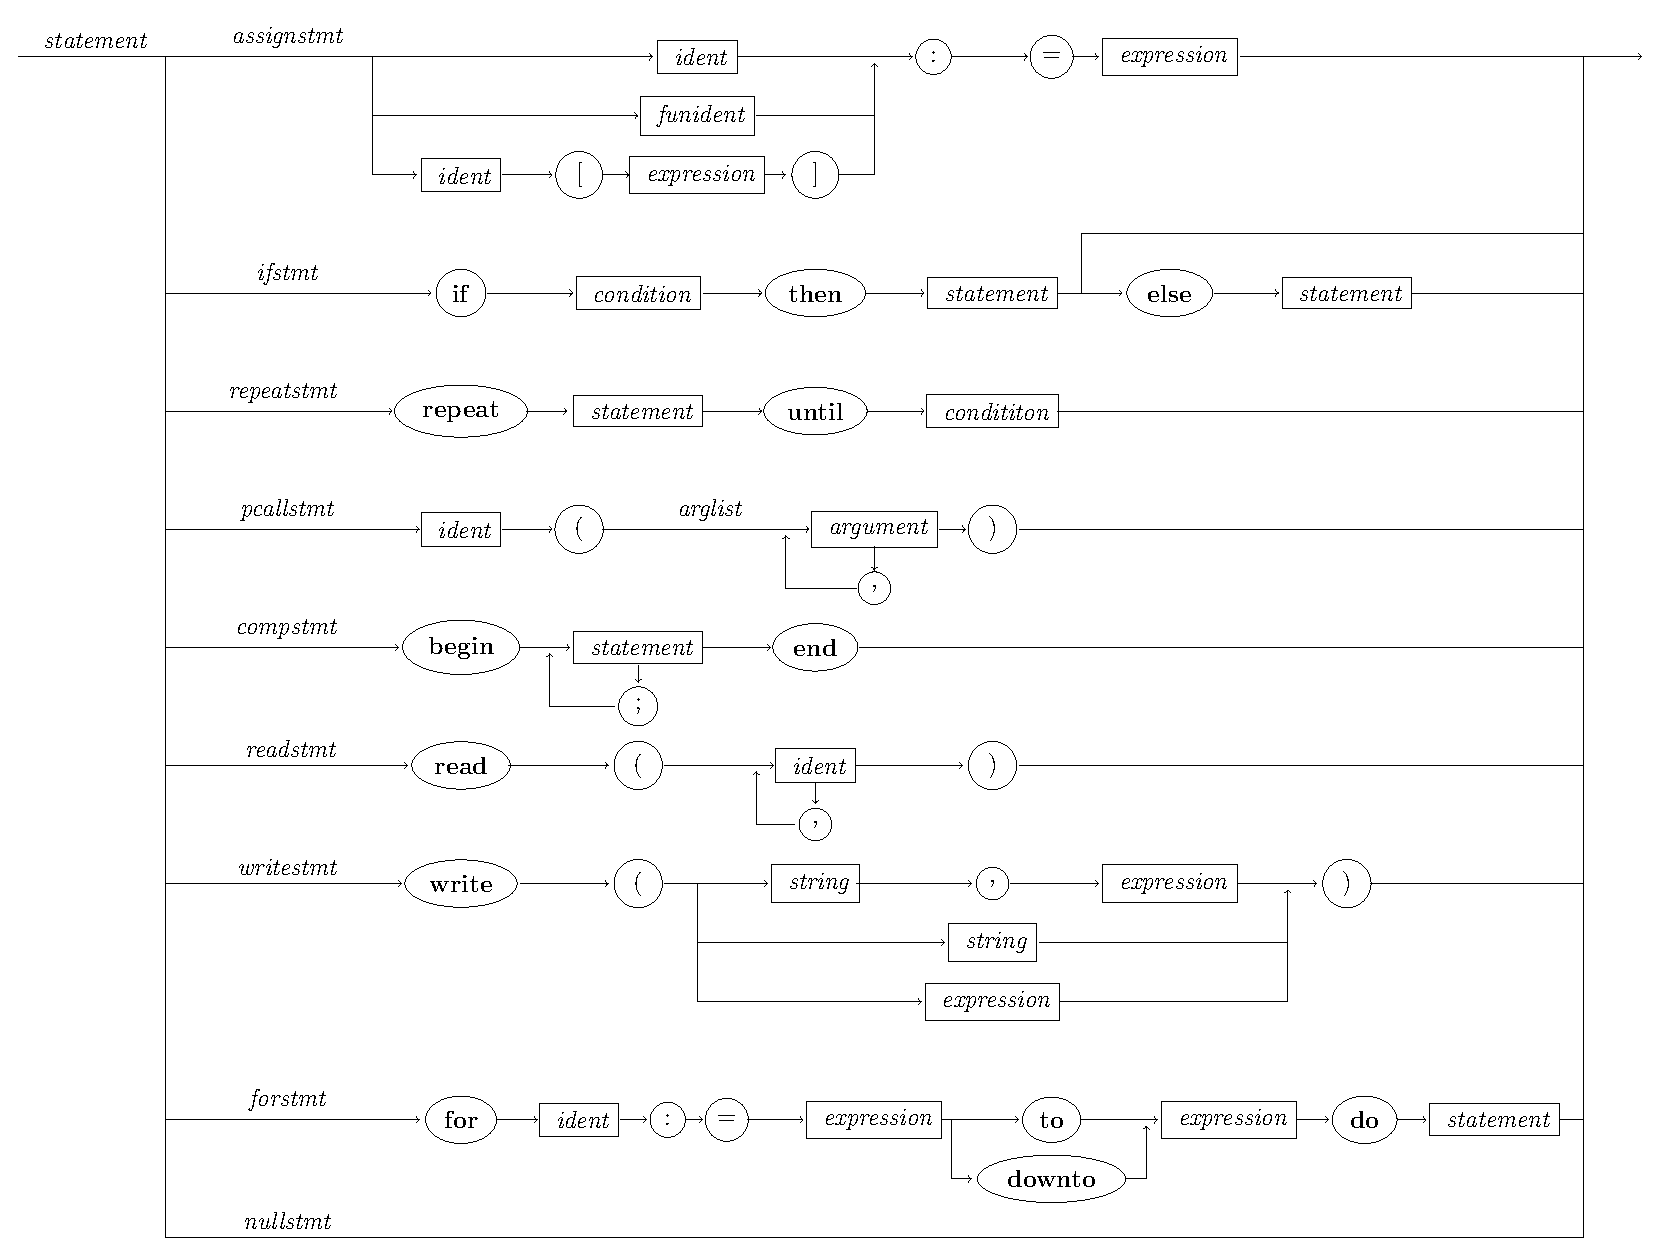
\includegraphics[scale=.6]{Figures/statement.eps}
\end{center}
\caption{statement 语法图}
\label{statement}
\end{figure}
具体实例:
\begin{verbatim}
const a=1, b=2, test=11, i=1;
var sum, k: integer; A:array[3] of of integer;
procedure testproc();
  testproc具体实现略;
begin
  // 赋值语句
  sum := a + b;
  A[i] := b;
  // 条件语句
  if a > b then
    sum := a;
  eles
    sum := b;
  // 重复语句
  repeat
    sum := sum + 1;
  until sum > 4
  // for语句 (步长为一)
  for i := 1 to 10 do
    sum := sum + i
  //过程调用语句
  testproc();
  //读语句
  read (k, sum);
  //写语句
  write("hello world!");
  write(sum)
end
\end{verbatim}
说明:
\begin{enumerate}
	\item 赋值语句可以是表达式给变量的赋值,可以是表达式给数组赋值,
		还可以给表达式给函数给返回值。
	\item 条件语句的\keyword{else}悬挂的解决方法是总将\keyword{else}
		和最近的\keyword{if}进行匹配。
	\item for语句的步长设为一,\keyword{to}表示变量值加一,\keyword{downto}
		表示变量值减一。
	\item 读语句,写语句和过程调用语句比较简单。
	\item 复合语句被\keyword{begin}和\keyword{end}围起来,之间是以
		分号隔开。
	\item 语句可以为空,即什么都没有。
\end{enumerate}
\subsection{类型的解读}
\[
	\sym{type} \define
		\sym{basictype} | \keyword{array} '['\sym{unsign}']' \keyword{of} \sym{basictype}
\]
\[
	\sym{basictype} \define
		\keyword{integer} | \keyword{char}
\]
\[
	\sym{const} \define
		[+|-]\sym{unsign}|\sym{character}
\]
\[
	\sym{character} \define
		'\sym{letter}' | '\sym{digit}'
\]
\[
	\sym{string} \define
		``\{ASCII~characters~with~decimal~code~number~varys~from~32~to~126~exclude~34\}"
\]
\[
	\sym{unsign} \define
		\sym{digit} \{\sym{digit}\}
\]
\[
	\sym{letter} \define
		a|b|c|...|z|A|B|C|...|Z
\]
\[
	\sym{digit} \define
		0|1|2|3|...|9
\]
类型的定义比较简单,就不画语法图了。直接说明。
\begin{enumerate}
	\item 具体的类型分为两类:基本类型和数组。
	\item 基本类型包括\keyword{integer}和\keyword{char}。整型
		包含正负的整数;char型包含数字位和大小写字母,定义时以单引号
		隔开。
	\item 字符串包含十进制ASCII码值从32到126的所有的值但是得剔除值为34的
		双引号。这样有利于词法分析的状态机的设计。另外字符串不是一种
		类型,只用于写语句的打印。
	\item 常量的定义可以是正负整数,也可以是字符。若是字符,则会使用ASCII
		码值进行运算。
\end{enumerate}
\subsection{表达式,项,因子的解读}
\subsubsection{表达式}
\[
	\sym{expression} \define
		[+|-] \sym{term} \{ \sym{addop} \sym{term} \}
\]
表达式的语法图见Figure~\ref{expression}。
下面是一些表达式的样例:
\begin{verbatim}
- 3 + a
a + b
1 - 10
a + 1 - 5
\end{verbatim}
\begin{figure}[h!]
\begin{center}
    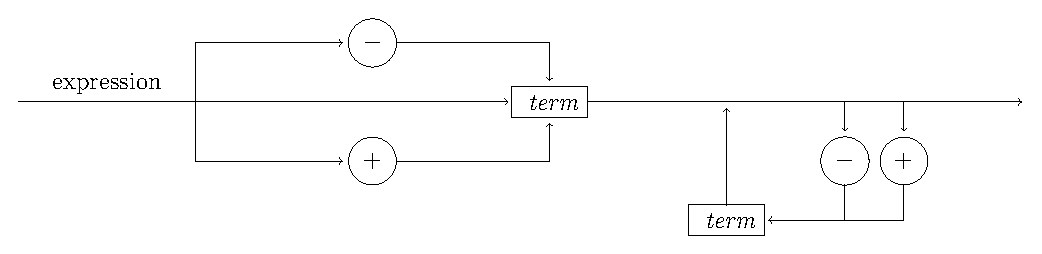
\includegraphics[scale=.8]{Figures/expression.eps}
\end{center}
\caption{expression 语法图}
\label{expression}
\end{figure}
\subsubsection{项}
\[
	\sym{term} \define
		\sym{factor} \{ \sym{multop} \sym{factor} \}
\]
项的语法图见Figure~\ref{term}。
下面是一些项的样例:
\begin{verbatim}
a * b
1 / 10
a / 1 * 5
\end{verbatim}
\begin{figure}[h!]
\begin{center}
    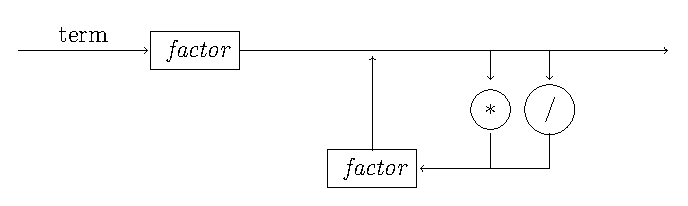
\includegraphics[scale=.8]{Figures/term.eps}
\end{center}
\caption{term 语法图}
\label{term}
\end{figure}
\subsubsection{因子}
\[
	\sym{factor} \define
		\sym{ident} | \sym{ident} '[' \sym{expression} ']' | \sym{unsign} |
			'(' \sym{expression} ')' | \sym{callstmt}
\]
\[
	\sym{fcallstmt} \define
		\sym{ident} '('[ \sym{arglist} ]')'
\]

因子的语法图见Figure~\ref{factor}。
下面是一些因子的样例:
\begin{verbatim}
const a = 1;
var A:array[3] of integer;
function somefun(): integer;
  somefun程序略;
// 下面的是因子
a 
A[2]
(a + b)
somefun()
\end{verbatim}
\begin{figure}[h!]
\begin{center}
    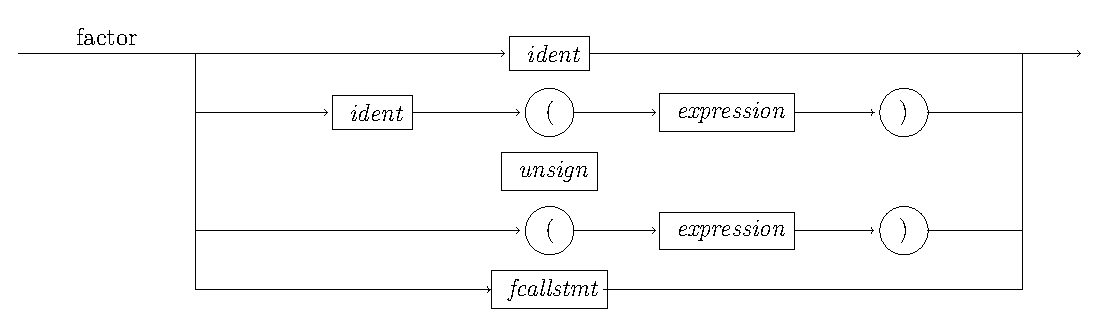
\includegraphics[scale=.8]{Figures/factor.eps}
\end{center}
\caption{factor 语法图}
\label{factor}
\end{figure}
\subsection{其他一些杂项}
\[
	\sym{ident} \define
		\sym{letter} \{ \sym{letter} | \sym{digit} \}
\]
\[
	\sym{paralist} \define
		[ \keyword{var} ] \sym{ident} \{, \sym{ident} \}: \sym{basictype} \{; \sym{paralist} \}
\]
\[
	\sym{funident} \define
		\sym{ident}
\]
\[
	\sym{arglist} \define
		\sym{argument} \{, \sym{argument} \}
\]
\[
	\sym{argument} \define
		\sym{expression}
\]
\[
	\sym{addop} \define
		+|-
\]
\[
	\sym{multop} \define
		*|/
\]
\[
	\sym{condition} \define
		\sym{expression} \sym{relop} \sym{expression}
\]
\[
	\sym{relop} \define
		< | <= | > | >=| = |  <>
\]
杂项的说明:
\begin{enumerate}
	\item 关于标识符的解析可以总结成一个状态机,见 Figure~\ref{getToken}
	\item 形参列表需要给出参数类型。
	\item 参数列表是由实参组成,之间使用逗号隔开。
	\item 实参被定义成一个表达式。
	\item 条件是基于一些比较,零表示假,非零表示真。
\end{enumerate}
\begin{figure}[!h]
\begin{center}
    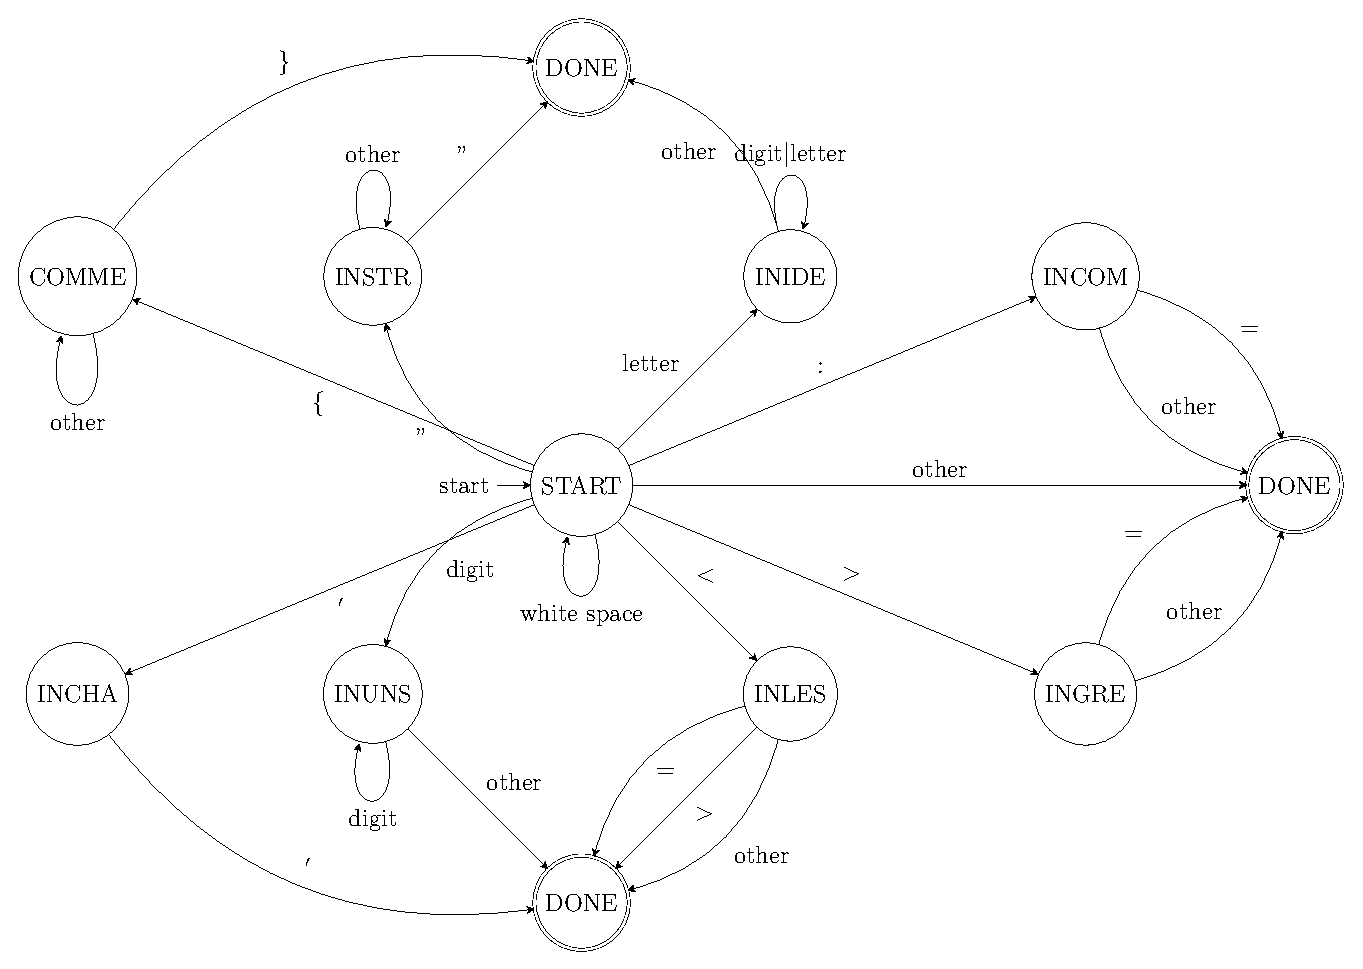
\includegraphics[scale=.8]{Figures/getToken.eps}
\end{center}
\caption{getToken 状态机}
\label{getToken}
\end{figure}

